\documentclass[12pt, a4paper, fleqn]{article}
\usepackage[utf8]{vietnam}
\usepackage{amsmath}
\usepackage{amsfonts}
\usepackage{amssymb}
\usepackage{cases}
\usepackage{tabularx}

\usepackage{scrextend}
\changefontsizes{13pt}

\usepackage{tikz}
\usetikzlibrary{calc}

\usepackage{graphicx}
\graphicspath{ {./images/} }

\setlength{\parindent}{0cm}
\setlength{\parskip}{0.1cm}
\setlength{\mathindent}{0pt}

\usepackage{geometry}
\geometry{
	a4paper,
	total = {160mm, 247mm},
	left = 25mm,
	top = 25mm,
}

\usepackage{listings}

\lstdefinestyle{mystyle}{
	basicstyle = \ttfamily\small,
	breakatwhitespace = false,
	breaklines = false,
	captionpos = b,
	keepspaces = false,
	showspaces = false,
	showstringspaces = false,
	showtabs = false,
	tabsize = 4,
	frame = single
}
\lstset{style = mystyle}

\usepackage{tocloft}
\renewcommand{\cftsecleader}{\cftdotfill{\cftdotsep}}
\setlength\cftaftertoctitleskip{30pt}

\usepackage{fancyhdr}
\pagestyle{fancy}
\fancyhf{}
\fancyhead[LE,RO]{CS112.K11}
\fancyhead[RE,LO]{\textit{[HW05] Phân tích thực nghiệm}}
\fancyfoot[CE,RO]{\thepage}

\usepackage{enumitem}

\begin{document}
	
	\begin{titlepage}
		   %Vẽ đường viền
		   \begin{tikzpicture}[overlay, remember picture]
				%Vẽ đường viền màu xanh
				\draw
					[blue!70!black, line width = 6pt]
					([xshift = -1.5cm, yshift = -2cm] current page.north east) coordinate (A) --
					([xshift = 1.5cm, yshift = -2cm] current page.north west) coordinate(B) --
					([xshift = 1.5cm, yshift = 2cm] current page.south west) coordinate (C) --
					([xshift = -1.5cm, yshift = 2cm] current page.south east) coordinate(D) -- cycle;
			
				%Vẽ đường viền màu đen
				\draw
					([yshift = 0.2cm, xshift = -0.2cm] A) --
					([yshift = 0.2cm, xshift = 0.2cm] B)--
					([yshift = -0.2cm, xshift = 0.2cm] B) --
					([yshift = -0.2cm, xshift = -0.2cm] B) --
					([yshift = 0.2cm, xshift = -0.2cm] C) --
					([yshift = 0.2cm, xshift = 0.2cm] C) --
					([yshift = -0.2cm, xshift = 0.2cm] C) --
					([yshift = -0.2cm, xshift = -0.2cm] D) --
					([yshift = 0.2cm, xshift = -0.2cm] D) --
					([yshift = 0.2cm, xshift = 0.2cm] D) --
					([yshift = -0.2cm, xshift = 0.2cm] A) --
					([yshift = -0.2cm, xshift = -0.2cm] B)--
					([yshift = 0.2cm, xshift = -0.2cm] B) --
					([yshift = 0.2cm, xshift = 0.2cm] B) --
					([yshift = -0.2cm, xshift = 0.2cm] C) --
					([yshift = -0.2cm, xshift = -0.2cm] C) --
					([yshift = 0.2cm, xshift = -0.2cm] C) --
					([yshift = 0.2cm, xshift = 0.2cm] D) --
					([yshift = -0.2cm, xshift = 0.2cm] D) --
					([yshift = -0.2cm, xshift = -0.2cm] D) --
					([yshift = 0.2cm, xshift = -0.2cm] A) --
					([yshift = 0.2cm, xshift = 0.2cm] A) --
					([yshift = -0.2cm, xshift = 0.2cm] A);
			\end{tikzpicture}
		
		%Thiết kế nội dung cho phần bìa
		\begin{center}
			\textbf{TRƯỜNG ĐẠI HỌC CÔNG NGHỆ THÔNG TIN}
			
			\vspace*{0.2cm}

			\textbf{KHOA KHOA HỌC MÁY TÍNH}
			
			\vspace*{0.2cm}
			
			\textbf{----------oOo----------}
			
			\vspace{1.5cm}
			
			
\includegraphics[width=0.25\textwidth]{UIT_Logo}
			
			\vspace{1.5cm}
			
			\Large
			\textbf{[HW05] PHÂN TÍCH THỰC NGHIỆM}
		
		\end{center}
			
			\vspace{3cm}
			\normalsize	
			
			\hspace{70pt} \textbf{\textit{Giảng viên hướng dẫn:}} ThS. Huỳnh Thị Thanh Thương\\
			
			\vspace*{1.5cm}
			
			\hspace{70pt} \textbf{\textit{Nhóm sinh viên:}}
			
			\vspace*{0.4cm}
			
			\hspace{70pt} 1. \hspace{10pt} Phan Thanh Hải  \hspace{45pt} 18520705
			
			\vspace{4cm}
		
		\begin{center}
			\textbf{TP. HỒ CHÍ MINH, 12/02/2020}
		\end{center}
			
	\end{titlepage}

	%Làm trang mục lục	
	\begin{center}
		\tableofcontents
	\end{center}
	\clearpage
	
	\setlength{\abovedisplayskip}{5pt}
	\setlength{\belowdisplayskip}{5pt}
	
	\setlist{noitemsep, topsep = 0pt, partopsep = 0pt, leftmargin = 0cm, labelindent = 0cm, itemindent = 1cm, align = left}
	
	\section*{Bài tập 1}
	
	\addcontentsline{toc}{section}{Bài tập 1}
	
	Dùng kỹ thuật toán sơ cấp để đếm số phép gán và số phép so sánh trong các đoạn chương trình sau. Sau đó suy ra độ phức tạp.
	
	Viết chương trình thực nghiệm để đếm số phép gán và số phép so sánh ở các câu trên, qua đó kiểm tra lại phần đếm lý thuyết.
	
	\subsection*{a.}
	
	\begin{lstlisting}[language = C++, mathescape]
float Alpha (float x, long n)
{	long i = 1; float z = 0;
	while (i $\leq$ n)
	{	long j = 1; float t = 1;
		while (j $\leq$ i)
		{	t = t*x;
			j = 2*j;
		}
		z = z + i*t;
		i = i + 1;
	}
	return z;
}
	\end{lstlisting}
	
	Gọi $\alpha_i$ là số lần lặp của vòng while trong (tính độc lập với vòng while ngoài).
	
	\begin{lstlisting}[language = C++, mathescape, texcl]
float Alpha (float x, long n)
{	long i = 1; float z = 0;			// 2 gán
	while (i $\leq$ n)						// n + 1 so sánh
	{	long j = 1; float t = 1;		// 2n gán
		while (j $\leq$ i)					// $\alpha_i$ + 1 so sánh
		{	t = t*x;					// $\alpha_i$ gán
			j = 2*j;					// $\alpha_i$ gán
		}
		z = z + i*t;					// n gán
		i = i + 1;						// n gán
	}
	return z;
}
	\end{lstlisting}
	
	Số phép gán:
	
	Gan$\displaystyle (n) = 2 + 4n + 2 \sum_{i = 1}^n \alpha_i$
	
	Số phép so sánh:
	
	SoSanh$\displaystyle (n) = n + 1 + \sum_{i = 1}^n (\alpha_i + 1)$
	
	Tính $\alpha_i$?
	\begin{align*}
		\alpha_i &= \text{số lần lặp của vòng while trong} \\
		         &= \text{số con $j$ chạy từ 1 đến $i$, bước tăng là $2j$} \\
		         &= \left| \{ 1; 2; 4; ...; 2^{k - 1} \} \right| \\
		         &= \left| \{ 2^{k - 1} | k \in \mathbb{N^*}, 1 \leq 2^{k - 1} \leq i\} \right| 
	\end{align*}
	
	Ta có:
	
	$1 \leq 2^{k - 1} \leq i \Leftrightarrow \log_2 1 \leq k - 1 \leq \log_2 i \Leftrightarrow 1 \leq k \leq \log_2 i + 1$
	
	Do đó $\alpha_i = \left\lfloor \log_2 i + 1 \right\rfloor$.
	
	Kết luận:
	
	Số phép gán:
	
	Gan$\displaystyle (n) = 2 + 4n + 2 \sum_{i = 1}^n \left\lfloor \log_2 i + 1 \right\rfloor$
	
	Số phép so sánh:
	
	SoSanh$\displaystyle (n) = n + 1 + \sum_{i = 1}^n \left\lfloor \log_2 i + 2 \right\rfloor$
	
	Vậy Gan$(n)$ + SoSanh$(n)$ = O$(n \log n)$.
	
	\subsection*{b.}
	
	\begin{lstlisting}[language = C++, mathescape]
float Omega (float x, long n)
{	long i = 1; float z = 0;
	while (i $\leq$ n)
	{	long j = 1; float t = 1;
		while (j $\leq$ i*i*i)
		{	t = t*x;
			j = j + 1;
		}
		z = z + i*t;
		i = 2*i;
	}
	return z;
}
\end{lstlisting}

	Gọi $\alpha_i$ là số lần lặp của vòng while ngoài.
	
	Tính $\alpha_i$?
	\begin{align*}
		\alpha_i &= \text{số lần lặp của vòng while ngoài} \\
				 &= \text{số con $i$ chạy từ 1 đến $n$, bước tăng là $2i$} \\
				 &= \left| \{ 1; 2; 4; ...; 2^{k - 1} \} \right| \\
				 &= \left| \{ 2^{k - 1} | k \in \mathbb{N^*}, 1 \leq 2^{k - 1} \leq n\} \right| 
	\end{align*}
	
	Ta có:
	
	$1 \leq 2^{k - 1} \leq n \Leftrightarrow \log_2 1 \leq k - 1 \leq \log_2 n \Leftrightarrow 1 \leq k \leq \log_2 n + 1$
	
	Do đó $\alpha_i = \left\lfloor \log_2 n + 1 \right\rfloor$.
	
	\begin{lstlisting}[language = C++, mathescape, texcl]
float Omega (float x, long n)
{	long i = 1; float z = 0;		// 2 gán
	while (i $\leq$ n)					// $\left\lfloor \log_2 n + 2 \right\rfloor$ so sánh
	{	long j = 1; float t = 1;	// $\left\lfloor 2 \log_2 n + 2 \right\rfloor$ gán
		while (j $\leq$ i*i*i)
		{	t = t*x;
			j = j + 1;
		}
		z = z + i*t;				// $\left\lfloor \log_2 n + 1 \right\rfloor$ gán
		i = 2*i;					// $\left\lfloor \log_2 n + 1 \right\rfloor$ gán
	}
	return z;
}
	\end{lstlisting}
	
	Xét độc lập vòng while trong với vòng while ngoài, ta có số phép gán gán và số phép so sánh lần lượt là $2i^3$ và $i^3 + 1$.
	
	Xét vòng while trong đặt trong vòng while ngoài, vì $i$ có bước tăng là $2i$ nên ta có:
	
	Với vòng lặp thứ 1 thì $i = 1$.
	
	Với vòng lặp thứ 2 thì $i = 1.2 = 2$.
	
	Với vòng lặp thứ 3 thì $i = 2.2 = 4$...
	
	Với vòng lặp thứ $k$ thì $i = 2^{k - 1}$.
	
	Có tất cả $\left\lfloor \log_2 n + 1 \right\rfloor$ lần lặp nên số phép gán và số phép so sánh lần lượt của vòng while trong là $\displaystyle 2 \sum_{i = 1}^{\left\lfloor \log_2 n + 1 \right\rfloor} 2^{3i - 3}$ và $\displaystyle \sum_{i = 1}^{\left\lfloor \log_2 n + 1 \right\rfloor} \left( 2^{3i - 3} + 1 \right)$.
	
	Kết luận:
	
	Số phép gán:
	\begin{align*}
		\text{Gan}(n) &= 2 + 4 \left\lfloor \log_2 n \right\rfloor + 4 + 2 \sum_{i = 1}^{\left\lfloor \log_2 n + 1 \right\rfloor} 2^{3i - 3} \\
					  &= 4 \left\lfloor \log_2 n \right\rfloor + 6 + \frac{2}{7}\left( 8^{\left\lfloor \log_2 n + 1 \right\rfloor} - 1 \right) \\
					  &= \frac{2}{7}\left( 8n^3 - 1 \right) + 4 \left\lfloor \log_2 n \right\rfloor + 6 \qquad \left( \text{với } n = 2^{\left\lfloor \log_2 n \right\rfloor} \right) 
	\end{align*}
	
	Số phép so sánh:
	\begin{align*}
		\text{SoSanh}(n) &= \left\lfloor \log_2 n \right\rfloor + 2 + \sum_{i = 1}^{\left\lfloor \log_2 n + 1 \right\rfloor} \left( 2^{3i - 3} + 1 \right) \\
						 &= \left\lfloor \log_2 n \right\rfloor + 2 + \frac{1}{7}\left( 8^{\left\lfloor \log_2 n + 1 \right\rfloor} - 1 \right) + \left\lfloor \log_2 n \right\rfloor + 1 \\
						 &= \frac{1}{7}\left( 8n^3 - 1 \right) + 2 \left\lfloor \log_2 n \right\rfloor + 3 \qquad \left( \text{với } n = 2^{\left\lfloor \log_2 n \right\rfloor} \right) 
	\end{align*}
	
	Vậy Gan$(n)$ + SoSanh$(n)$ = O$(n^3)$.
	
	\subsection*{c.}
	
	\begin{lstlisting}[language = C++, mathescape]
i = 1; ret = 0; s = 0;
while (i $\leq$ n)
{	j = 1;
	s = s + 1/i;
	while (j $\leq$ s)
	{	ret = ret + i*j;
		j = j + 1;
	}
	i = i + 1;
}
\end{lstlisting}
	
	Gọi $\alpha_i$ là số lần lặp của vòng while trong (tính độc lập với vòng while ngoài).
	
	\begin{lstlisting}[language = C++, mathescape, texcl]
i = 1; ret = 0; s = 0; 			// 3 gán
while (i $\leq$ n)					// n + 1 so sánh
{	j = 1;						// n gán
	s = s + 1/i;				// n gán
	while (j $\leq$ s)				// $\alpha_i$ + 1 so sánh
	{	ret = ret + i*j;		// $\alpha_i$ gán
		j = j + 1;				// $\alpha_i$ gán
	}
	i = i + 1;					// n gán
}
	\end{lstlisting}
	
	Số phép gán:
	
	Gan$\displaystyle (n) = 3 + 3n + 2 \sum_{i = 1}^n \alpha_i$
	
	Số phép so sánh:
	
	SoSanh$\displaystyle (n) = n + 1 + \sum_{i = 1}^n (\alpha_i + 1)$
	
	Tính $\alpha_i$?
	\begin{align*}
	\alpha_i &= \text{số lần lặp của vòng while trong} \\
			 &= \text{số con $j$ chạy từ 1 đến $s$, bước tăng là $j + 1$} 
	\end{align*}
	
	Ta có:
	
	$\displaystyle s_i = s_{i - 1} + \frac{1}{i} = s_{i - 2} + \frac{1}{i - 1} + \frac{1}{i} = ... = 1 + \frac{1}{2} + ... + \frac{1}{i} = \sum_{k = 1}^i \frac{1}{k}$
	
	Do đó $\displaystyle \alpha_i = \sum_{k = 1}^i \frac{1}{k}$.
	
	Kết luận:
	
	Số phép gán:
	
	Gan$\displaystyle (n) = 3 + 3n + 2 \sum_{i = 1}^n \sum_{k = 1}^i \frac{1}{k}$
	
	Số phép so sánh:
	
	SoSanh$\displaystyle (n) = n + 1 + \sum_{i = 1}^n \left( \sum_{k = 1}^i \frac{1}{k} + 1 \right) $
	
	Vậy Gan$(n)$ + SoSanh$(n)$ = O$(n \log n)$.

	\subsection*{d.}
	
	\begin{lstlisting}[language = C++, mathescape]
i = 1;
count = 0;
while (i $\leq$ 3*n)
{
	x = 2*n - i;
	y = i - n;
	j = 1;
	while (j $\leq$ x)
	{
		if (j $\geq$ n)
			count = count - 1;
		j = j + 1;
	}
	if (y > 0)
		if (x > 0)
			count = count + 1;
	i = i + 1;
}
\end{lstlisting}

	Gọi $\alpha_i$ là số lần lặp của vòng while trong (tính độc lập với vòng while ngoài).
	
	\begin{lstlisting}[language = C++, mathescape, texcl]
i = 1;							// 1 gán
count = 0;						// 1 gán
while (i $\leq$ 3*n)					// 3n + 1 so sánh
{
	x = 2*n - i;				// 3n gán
	y = i - n;					// 3n gán
	j = 1;						// 3n gán
	while (j $\leq$ x)				// $\alpha_i$ + 1 so sánh
	{
		if (j $\geq$ n)				// $\alpha_i$ so sánh
			count = count - 1;	// (*)
		j = j + 1;				// $\alpha_i$ gán
	}
	if (y > 0)					// 3n so sánh
		if (x > 0)				// (**)
			count = count + 1;	// (***)
	i = i + 1;					// 3n gán
}
	\end{lstlisting}
	
	Tính $\alpha_i$?
	\begin{align*}
		\alpha_i &= \text{số lần lặp của vòng while trong} \\
				 &= \text{số con $j$ chạy từ 1 đến $x$, bước tăng là $j + 1$} \\
				 &= x - 1 + 1 = 2n - i
	\end{align*}
	
	Vòng lặp while trong chỉ được thực hiện $\Leftrightarrow x \geq 1 \Leftrightarrow 2n - i \geq 1 \Leftrightarrow i \leq 2n - 1$ \\

	Số lần thực hiện lệnh (*) = số con $j$ lớn hơn hoặc bằng $n$
	
	Mà $j$ đi từ 1 đến $2n - i$
	
	Do đó, số lần thực hiện lệnh (*) = $(2n - i) - n + 1 = n - i + 1$, với $i \leq n$.
	
	Xét số lần thực hiện lệnh (**) và (***). Ta có:
	\begin{center}
		\begin{tabular}{ | m {2.2 cm} | m {12.8 cm} | } 
			\hline
			\hspace*{25pt} $i$ & 0 \hspace*{105pt} $n$ \hspace*{105pt} $2n$ \hspace*{90pt} $3n$ \\
			\hspace*{2pt} $y = i - n$ & \hspace*{49pt} $-$ \hspace*{49pt} 0 \hspace*{50pt} + \hspace*{100pt} + \\
			\hspace*{1pt} $x = 2n - i$ & \hspace*{49pt} + \hspace*{114pt} + \hspace*{40pt} 0 \hspace*{45pt} $-$ \\
			\hline
		\end{tabular}
	\end{center}
	\begin{align*}
	\text{Số lần thực hiện lệnh (**)} &= \text{số con $i$ làm cho $y > 0$} \\
							   		  &= \text{số con $i$ đi từ $n + 1$ đến $3n$} \\
								   	  &= 3n - (n + 1) + 1 = 2n.
	\end{align*}
	\begin{align*}
	\text{Số lần thực hiện lệnh (***)} &= \text{số con $i$ làm cho $y > 0$ và $x > 0$} \\
									   &= \text{số con $i$ đi từ $n + 1$ đến $2n - 1$} \\
									   &= (2n - 1) - (n + 1) + 1 = n - 1.
	\end{align*}
	Kết luận:
	
	Số phép gán:
	\begin{align*}
	\text{Gan}(n) &= 2 + 12n + (n - 1) + \sum_{i = 1}^{n} (n - i + 1) + \sum_{i = 1}^{2n - 1} (2n - i) \\
				  &= 13n + 1 + \frac{1}{2} n(n + 1) + n(2n - 1) = \frac{5}{2}n^2 + \frac{25}{2}n + 1
	\end{align*}
	
	Số phép so sánh:
	\begin{align*}
	\text{SoSanh}(n) &= 3n + 1 + 3n + 2n + \sum_{i = 1}^{2n - 1} [(2n - i + 1) + (2n - i)] + \sum_{i = 2n}^{3n} 1 \\
					 &= 8n + 1 + \sum_{i = 1}^{2n - 1} (4n - 2i + 1) + (n + 1) \\
					 &= 8n + 1 + (4n^2 - 1) + (n + 1) = 4n^2 + 9n + 1
	\end{align*}
	
	Vậy Gan$(n)$ + SoSanh$(n)$ = O$(n^2)$.
	
	\clearpage

	\section*{Bài tập 2}
	
	\addcontentsline{toc}{section}{Bài tập 2}
	
	Phân tích độ phức tạp của thuật toán binary search (tìm kiếm nhị phân) trong trường hợp worst case. Với thuật toán binary search mỗi input là một mảng số nguyên \textbf{có thứ tự} và một số nguyên cần tìm. Độ dài của mảng được xem là kích thước của input. Trường hợp worst case của binary search là khi số này không có trong mảng.
	\begin{itemize}
		\item Phân tích dựa trên thời gian thực thi, trường hợp worst case.
		\item Mẫu thử nghiệm (sample) có ít nhất 30 trường hợp (instance) với kích thước khác nhau.
		\item Trường hợp nhỏ nhất có kích thước 100 phần tử.
		\item Trường hợp sau kích thước lớn hơn trường hợp trước 50\%.
		\item Ứng với mỗi trường hợp phát sinh 10 input với giá trị ngẫu nhiên khác nhau và tính thời gian trung bình cho 10 trường hợp này.
	\end{itemize}
	
	\subsection*{a. Thuật toán}
	
	\textbf{BinarySearch}$(A[0..n - 1, x])$	
	
	\begin{enumerate}
		\item $l = 0$;
		\item $r = n - 1$;
		\item \textbf{while} $l \leq r$ \textbf{do}
		\item \qquad $m = (l + r) / 2$;
		\item \qquad \textbf{if} $x = A[m]$
		\item \qquad \qquad \textbf{return} $m$;
		\item \qquad \textbf{else}
		\item \qquad \qquad \textbf{if} $x < A[m]$
		\item \qquad \qquad \qquad $r = m - 1$;
		\item \qquad \qquad \textbf{else}
		\item \qquad \qquad \qquad $l = m + 1$;
		\item \textbf{return} $-1$;
	\end{enumerate}

	Trường hợp worst case của binary search là khi số cần tìm không có trong mảng.
	
	\subsection*{b. Cách phát sinh dữ liệu thử nghiệm}
	
	Mẫu thử nghiệm (sample) có 30 trường hợp (instance) với kích thước khác nhau.
	
	Trường hợp nhỏ nhất có kích thước 100 phần tử.
	
	Trường hợp sau kích thước lớn hơn trường hợp trước 50%.
	
	Ứng với mỗi trường hợp phát sinh 10 input với giá trị ngẫu nhiên khác nhau, mỗi input là một mảng mà các giá trị trong mảng đi từ 0 đến 999999 và số cần tìm $x$ (giá trị của số cần tìm $x$ cũng đi từ 0 đến 999999).
	
	Khi phát sinh giá trị ngẫu nhiên trong mảng ta sẽ đánh dấu giá trị đó và khi phát sinh giá trị ngẫu nhiên cho số cần tìm $x$, ta kiểm tra giá trị đó đã được đánh dấu chưa. Nếu đã đánh dấu thì ta phát sinh lại giá trị ngẫu nhiên cho số cần tìm $x$ cho đến khi giá trị của nó chưa được đánh dấu trong mảng.
	
	\subsection*{c. Cách tiến hành thử nghiệm}
	
	Phân tích dựa trên thời gian thực thi, trường hợp worst case.
	
	Thời gian thực thi được tính bằng giây, xác định bằng hiệu thời gian hoàn tất gọi hàm $t_{finish}$ và thời gian bắt đầu gọi hàm $t_{start}$.
	
	Ta sẽ viết chương trình tự nhập input và xuất thời gian thực thi ra màn hình. Sau đó copy output vào file Excel.
	
	Dựa vào kết quả output trong file Excel, ta tính thời gian trung bình cho mỗi trường hợp tương ứng và xuất kết quả vào file text.
	
	\subsection*{d. Cấu hình máy chạy thử nghiệm}
	
	$$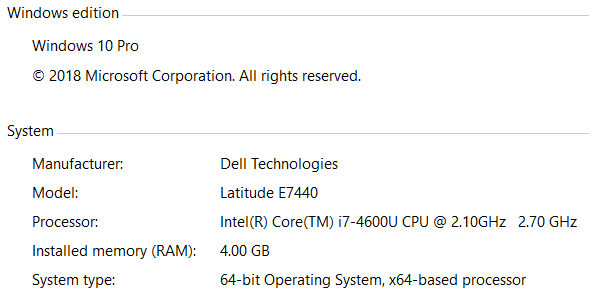
\includegraphics[width=0.9\textwidth]{Cau_hinh}$$
	
	\subsection*{e. Phân tích và kết luận độ phức tạp của thuật toán}
	
	Ta sẽ vẽ biểu đồ dựa vào dữ liệu thử nghiệm đã thu được.
	$$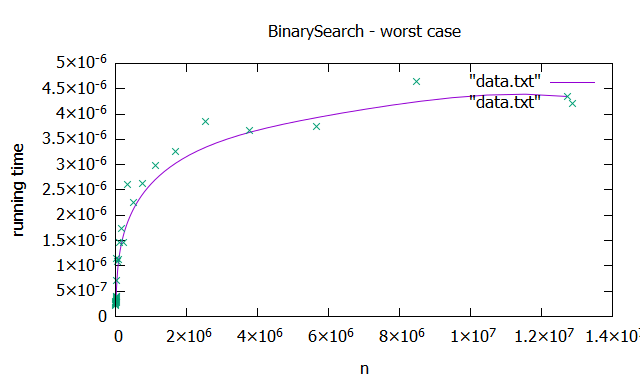
\includegraphics[width=0.9\textwidth]{Exercise2}$$
	
	Dựa vào biểu đồ, ta dự đoán độ phức tạp của thuật toán binary search trong trường hợp trung bình là O$(\log n)$.
	
	\clearpage
	
	\section*{Bài tập 3}
	
	\addcontentsline{toc}{section}{Bài tập 3}
	
	Phân tích thuật toán quick sort trong trường hợp worst case.
	\begin{itemize}
		\item Phân tích dựa trên \textbf{số phép so sánh}, trường hợp worst case.
		\item Mẫu thử nghiệm (sample) có ít nhất 40 trường hợp (instance) với kích thước khác nhau.
		\item Trường hợp nhỏ nhất có kích thước 10 phần tử.
		\item Trường hợp sau kích thước lớn hơn trường hợp trước 30\%.
	\end{itemize}
	
	\subsection*{a. Thuật toán}
	
	\textbf{LomutoPartition}$(A[0..n - 1, l, r])$	
	
	\begin{enumerate}
		\item $pivot = A[r]$;
		\item $i = l - 1$;
		\item \textbf{for} $j = l$ \textbf{to} $r - 1$ \textbf{do}
		\item \qquad \textbf{if} $A[j] \leq pivot$
		\item \qquad \qquad$i = i + 1$;
		\item \qquad \qquad Hoán vị phần tử $A[i]$ với $A[j]$;
		\item Hoán vị phần tử $A[i + 1]$ với $A[r]$;
		\item \textbf{return} $i + 1$; \\
	\end{enumerate}
	
	\textbf{QuickSort}$(A[0..n - 1, l, r])$
	
	\begin{enumerate}
		\item \textbf{if} $l < r$
		\item \qquad $p$ = \textbf{LomutoPartition}$(A, p, r)$;
		\item \qquad \textbf{QuickSort}$(A, l, p - 1)$;
		\item \qquad \textbf{QuickSort}$(A, p + 1, r)$;
	\end{enumerate}

	Trường hợp worst case của quick sort là khi quá trình phân hoạch mất cân bằng tại mỗi bước phân hoạch, nghĩa là: dãy phân hoạch một phần chỉ có 1 phần tử và phần còn lại gồm có $n - 1$ phần tử.
	
	Thông thường, trường hợp worst case xảy ra khi input có một trong các đặc điểm sau:
	
	\begin{enumerate}
		\item Input đã được sắp xếp sẵn (tăng dần hoặc giảm dần).
		\item Các phần tử trong input có giá trị như nhau.
	\end{enumerate}

	\subsection*{b. Cách phát sinh dữ liệu thử nghiệm}
	
	Mẫu thử nghiệm (sample) có 40 trường hợp (instance) với kích thước khác nhau.
	
	Trường hợp nhỏ nhất có kích thước 10 phần tử.
	
	Trường hợp sau kích thước lớn hơn trường hợp trước 30%.
	
	Ứng với mỗi trường hợp phát sinh một input là một mảng mà các giá trị trong mảng đi từ 0 đến 9999.
	
	Để dữ liệu thử nghiệm khiến cho thuật toán quick sort rơi vào trường hợp worst case thì ta sẽ tiến hành sắp xếp mảng trước khi gọi hàm \textbf{QuickSort}.
	
	\subsection*{c. Cách tiến hành thử nghiệm}
	
	Phân tích dựa trên thời gian số phép so sánh, trường hợp worst case.
	
	Số phép so sánh của thuật toán QuickSort được tính bằng tổng số phép so sánh được thực hiện tại dòng 4 của hàm \textbf{LomutoPartition} và dòng 1 của hàm \textbf{QuickSort}.
	
	Ta sẽ viết chương trình tự nhập input và xuất số phép so sánh ra màn hình. Sau đó copy output vào file Excel.
	
	Dựa vào kết quả output trong file Excel, ta xuất kết quả vào file text.
	
	\subsection*{d. Cấu hình máy chạy thử nghiệm}
	
	$$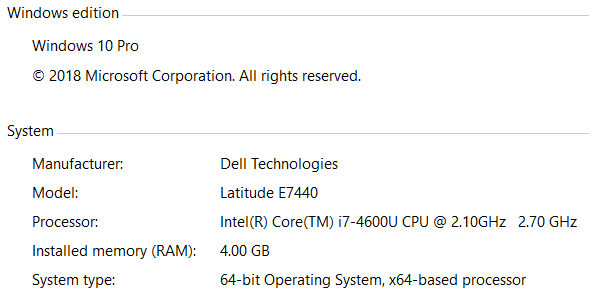
\includegraphics[width=0.9\textwidth]{Cau_hinh}$$
	
	\subsection*{e. Phân tích và kết luận độ phức tạp của thuật toán}
	
	Ta sẽ vẽ biểu đồ dựa vào dữ liệu thử nghiệm đã thu được.
	$$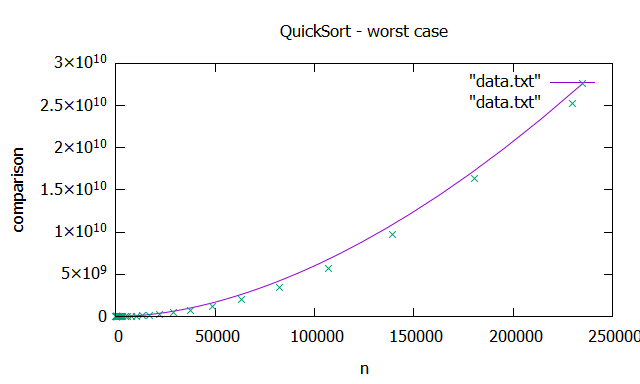
\includegraphics[width=0.9\textwidth]{Exercise3}$$
	
	Dựa vào biểu đồ, ta dự đoán độ phức tạp của thuật toán quick sort trong trường hợp worst case là O$(n^2)$.
	
	\clearpage
	
	\section*{Bài tập 4}
	
	\addcontentsline{toc}{section}{Bài tập 4}
	
	Phân tích thuật toán quick sort trong trường hợp average case.
	\begin{itemize}
		\item Phân tích dựa trên số thời gian chạy, trường hợp average case.
		\item Mẫu thử nghiệm (sample) có ít nhất 50 trường hợp (instance) với kích thước khác nhau.
		\item Trường hợp nhỏ nhất có kích thước 10 phần tử.
		\item Trường hợp sau kích thước lớn hơn trường hợp trước 30\%.
	\end{itemize}

	\subsection*{a. Thuật toán}
	
	\textbf{LomutoPartition}$(A[0..n - 1, l, r])$	
	
	\begin{enumerate}
		\item $pivot = A[r]$;
		\item $i = l - 1$;
		\item \textbf{for} $j = l$ \textbf{to} $r - 1$ \textbf{do}
		\item \qquad \textbf{if} $A[j] \leq pivot$
		\item \qquad \qquad$i = i + 1$;
		\item \qquad \qquad Hoán vị phần tử $A[i]$ với $A[j]$;
		\item Hoán vị phần tử $A[i + 1]$ với $A[r]$;
		\item \textbf{return} $i + 1$; \\
	\end{enumerate}
	
	\textbf{QuickSort}$(A[0..n - 1, l, r])$
	
	\begin{enumerate}
		\item \textbf{if} $l < r$
		\item \qquad $p$ = \textbf{LomutoPartition}$(A, p, r)$;
		\item \qquad \textbf{QuickSort}$(A, l, p - 1)$;
		\item \qquad \textbf{QuickSort}$(A, p + 1, r)$;
	\end{enumerate}

	\subsection*{b. Cách phát sinh dữ liệu thử nghiệm}
	
	Mẫu thử nghiệm (sample) có 50 trường hợp (instance) với kích thước khác nhau.
	
	Trường hợp nhỏ nhất có kích thước 10 phần tử.
	
	Trường hợp sau kích thước lớn hơn trường hợp trước 30\%.
	
	Ứng với mỗi trường hợp phát sinh 10 input với giá trị ngẫu nhiên khác nhau, mỗi input là một mảng mà các giá trị trong mảng đi từ 0 đến 99999.
	
	\subsection*{c. Cách tiến hành thử nghiệm}
	
	Phân tích dựa trên số thời gian chạy, trường hợp average case.
	
	Thời gian chạy được tính bằng giây, xác định bằng hiệu thời gian hoàn tất gọi hàm $t_{finish}$ và thời gian bắt đầu gọi hàm $t_{start}$.
	
	Ta sẽ viết chương trình tự nhập input và xuất thời gian chạy ra màn hình. Sau đó copy output vào file Excel.
	
	Dựa vào kết quả output trong file Excel, ta tính thời gian trung bình cho mỗi trường hợp tương ứng và xuất kết quả vào file text.
	
	\subsection*{d. Cấu hình máy chạy thử nghiệm}
	
	$$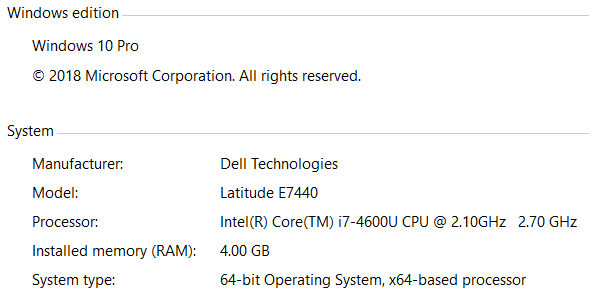
\includegraphics[width=0.9\textwidth]{Cau_hinh}$$
	
	\subsection*{e. Phân tích và kết luận độ phức tạp của thuật toán}
	
	Ta sẽ vẽ biểu đồ dựa vào dữ liệu thử nghiệm đã thu được.
	$$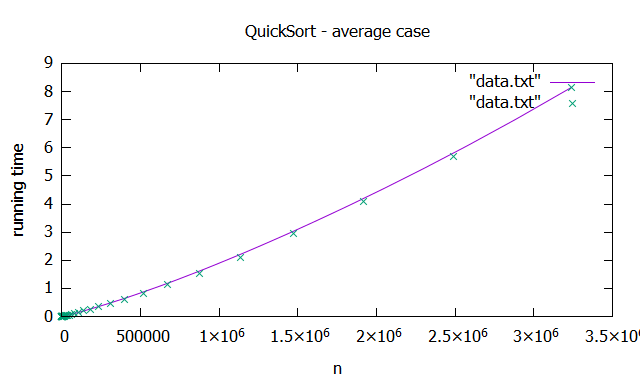
\includegraphics[width=0.9\textwidth]{Exercise4}$$
	
	Dựa vào biểu đồ, ta dự đoán độ phức tạp của thuật toán quick sort trong trường hợp average case là O$(n \log n)$.
	
	\clearpage
	
	\section*{Bài tập 5}
	
	\addcontentsline{toc}{section}{Bài tập 5}
	
	Phân tích thuật toán shell sort trong trường hợp average case.
	\begin{itemize}
		\item Phân tích dựa trên số thời gian chạy, trường hợp average case.
		\item Mẫu thử nghiệm (sample) có ít nhất 50 trường hợp (instance) với kích thước khác nhau.
		\item Trường hợp nhỏ nhất có kích thước 10 phần tử.
		\item Trường hợp sau kích thước lớn hơn trường hợp trước 30\%.
	\end{itemize}

	\subsection*{a. Thuật toán}

	\textbf{ShellSort}$(A[0..n - 1])$	
	
	\begin{enumerate}
		\item $gap = n/2$;
		\item \textbf{while} $gan > 0$ \textbf{do}
		\item \qquad \textbf{for} $i = gap$ \textbf{to} $n - 1$ \textbf{do}
		\item \qquad \qquad $temp = A[i]$;
		\item \qquad \qquad $j = i$;
		\item \qquad \qquad \textbf{while} $j \geq gap$ \textbf{and} $A[j - gap] > temp$ \textbf{do}
		\item \qquad \qquad \qquad $A[j] = A[j - gap]$;
		\item \qquad \qquad \qquad $j = j - gap$;
		\item \qquad \qquad $A[j] = temp$;
		\item \qquad $gap = gap / 2$;
	\end{enumerate}

	\subsection*{b. Cách phát sinh dữ liệu thử nghiệm}
	
	Mẫu thử nghiệm (sample) có 50 trường hợp (instance) với kích thước khác nhau.
	
	Trường hợp nhỏ nhất có kích thước 100 phần tử.
	
	Trường hợp sau kích thước lớn hơn trường hợp trước 30\%.
	
	Ứng với mỗi trường hợp phát sinh 10 input với giá trị ngẫu nhiên khác nhau, mỗi input là một mảng mà các giá trị trong mảng đi từ 0 đến 99999.
	
	\subsection*{c. Cách tiến hành thử nghiệm}
	
	Phân tích dựa trên số thời gian chạy, trường hợp average case.
	
	Thời gian chạy được tính bằng giây, xác định bằng hiệu thời gian hoàn tất gọi hàm $t_{finish}$ và thời gian bắt đầu gọi hàm $t_{start}$.
	
	Ta sẽ viết chương trình tự nhập input và xuất thời gian ra màn hình. Sau đó copy output vào file Excel.
	
	Dựa vào kết quả output trong file Excel, ta tính thời gian trung bình cho mỗi trường hợp tương ứng và xuất kết quả vào file text.
	
	\subsection*{d. Cấu hình máy chạy thử nghiệm}
	
	$$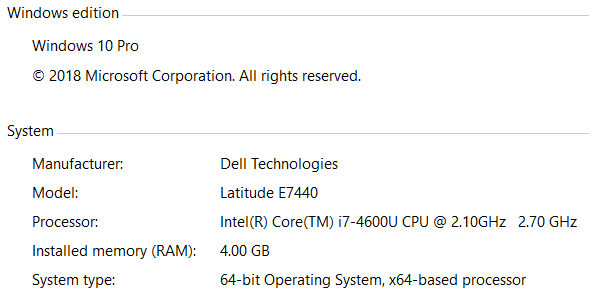
\includegraphics[width=0.9\textwidth]{Cau_hinh}$$
	
	\subsection*{e. Phân tích và kết luận độ phức tạp của thuật toán}
	
	Ta sẽ vẽ biểu đồ dựa vào dữ liệu thử nghiệm đã thu được.
	$$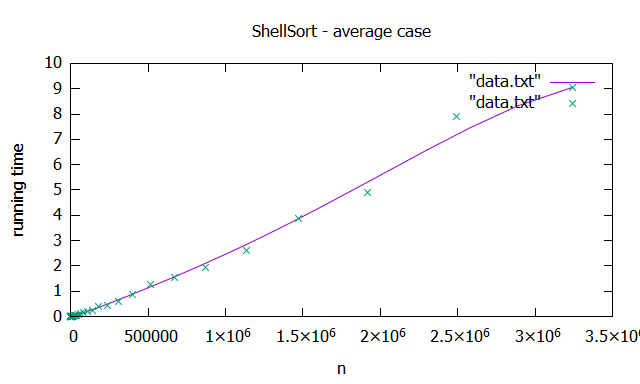
\includegraphics[width=0.9\textwidth]{Exercise5}$$
	
	Dựa vào biểu đồ, ta dự đoán độ phức tạp của thuật toán shell sort trong trường hợp average case là O$(n^2)$.
	
	\clearpage
	
	\section*{Bài tập 6}
	
	\addcontentsline{toc}{section}{Bài tập 6}
	
	Với mỗi $n$ nguyên dương, xem 2 thuật toán viết bằng mã giả sau đây:

	Thuật toán 1.
	
	\begin{lstlisting}[language = C++, mathescape]
i = 1; m = n - n*(n mod 2);
s = 3;
while (i $\leq$ m)
{	j = 1;
	k = i*i*(i mod 2);
	s = s + 3;
	while (j $\leq$ k)
	{	j = j + 1;
		s = s + 2;
	}
	i = i + 1;
	s = s + 2;
}
	\end{lstlisting}
	
	Thuật toán 2.
	
	\begin{lstlisting}[language = C++, mathescape]
i = 1; m = n*(n mod 2);
s = 3;
while (i $\leq$ m)
{	j = 1;
	k = i*i - i*i*(i mod 2);
	s = s + 3;
	while (j $\leq$ k)
	{	j = j + 1;
		s = s + 2;
	}
	i = i + 1;
	s = s + 2;
}
	\end{lstlisting}
	
	Giả sử ta chỉ quan tâm đến số phép gán và số phép so sánh được thực hiện trong mỗi thuật toán. Gọi Gan1$(n)$, SoSanh1$(n)$, Gan2$(n)$, SoSanh2$(n)$ lần lượt là số phép gán và số phép so sánh của thuật toán 1 và 2.
	
	\subsection*{a.}
	
	Tính theo $n$ số phép gán trong mỗi thuật toán. \\
	
	\textbf{Xét thuật toán 1.}
	
	a. Nếu $n$ là số lẻ thì $m = n - n*(n \mod 2) = n - n = 0$.
	
	Khi đó vào điều kiện trong vòng while ngoài thì điều kiện $i \leq m$ $(1 \leq 0)$ là sai, nên không thực hiện vòng lặp while ngoài.
	
	Do đó, với $n$ là số lẻ thì số phép gán là Gan1$(n)$ = 3.
	
	b. Nếu $n$ là số chẵn thì $m = n - n*(n \mod 2) = n - 0 = n$.
	
	Gọi $\alpha_i$ là số lần lặp của vòng while trong (tính độc lập với vòng while ngoài).
	
	\begin{lstlisting}[language = C++, mathescape, texcl]
i = 1; m = n - n*(n mod 2);			// 2 gán
s = 3;								// 1 gán
while (i $\leq$ m)						// n + 1 so sánh
{	j = 1;							// n gán
	k = i*i*(i mod 2);				// n gán
	s = s + 3;						// n gán
	while (j $\leq$ k)					// $\alpha_i$ + 1 so sánh
	{	j = j + 1;					// $\alpha_i$ gán
		s = s + 2;					// $\alpha_i$ gán
	}
	i = i + 1;						// n gán
	s = s + 2;						// n gán
}
	\end{lstlisting}
	
	Tính $\alpha_i$?
	\begin{align*}
	\alpha_i &= \text{số lần lặp của vòng while trong} \\
			 &= \text{số con $j$ chạy từ 1 đến $k$, bước tăng là $j + 1$}
	\end{align*}
	Ta có:
	
	Với $i$ là số lẻ $(i = 2a - 1, a \geq 1)$ thì $k = i*i*(i \mod 2) = i^2$.
	
	Khi đó thì $\alpha_i = i^2 = (2a - 1)^2$.
	
	Với $i$ là số chẵn thì $k = i*i*(i \mod 2) = 0$. Khi đó thì $\alpha_i = 0$.
	
	Do đó, với $n$ là số chẵn thì số phép gán là
	\begin{align*}
	\text{Gan1}(n) &= 3 + 5n + 2 \sum_{i = 1}^{\frac{n}{2}} (2i - 1)^2 \\
				   &= 3 + 5n + \frac{1}{3} n(n^2 - 1)
	\end{align*}
	
	Vậy Gan1$(n) = {
		\begin{cases}
		3 & {\text{nếu $n$ lẻ}} \\
		\displaystyle 3 + 5n + \frac{1}{3} n(n^2 - 1) & {\text{nếu $n$ chẵn}}
		\end{cases}
	}$

	\hfill \break

	\textbf{Xét thuật toán 2.}
	
	Thuật toán 2 chỉ có thay đổi giá trị $m$ và $k$ tùy theo giá trị của $n$ và $i$ là chẵn hay lẻ, còn lại làm tương tự như thuật toán 1.
	
	Vậy Gan2$(n) = {
		\begin{cases}
		3 & {\text{nếu $n$ chẵn}} \\
		\displaystyle 3 + 5n + \frac{1}{3} n(n^2 - 1) & {\text{nếu $n$ lẻ}}
		\end{cases}
	}$
	
	\subsection*{b.}
	
	Tính theo $n$ số phép so sánh trong mỗi thuật toán. \\
	
	\textbf{Xét thuật toán 1.}
	
	a. Nếu $n$ là số lẻ thì $m = n - n*(n \mod 2) = n - n = 0$.
	
	Khi đó vào điều kiện trong vòng while ngoài thì điều kiện $i \leq m$ $(1 \leq 0)$ là sai, nên không thực hiện vòng lặp while ngoài.
	
	Do đó, với $n$ là số lẻ thì số phép gán là SoSanh1$(n)$ = 1.
	
	b. Nếu $n$ là số chẵn thì $m = n - n*(n \mod 2) = n - 0 = n$.
	
	Sử dụng kết quả đã có ở câu a), ta được:
	
	Với $n$ là số chẵn thì số phép so sánh là
	\begin{align*}
	\text{SoSanh1}(n) &= n + 1 + \sum_{i = 1}^{\lceil \frac{n}{2} \rceil} \left[ (2i - 1)^2 + 1 \right] + \sum_{i = 1}^{\lfloor \frac{n}{2} \rfloor} 1 \\
					  &= n + 1 + \left\lceil \frac{1}{6} n(n^2 + 2) \right\rceil + \frac{1}{2} n \\
					  &= 1 + \frac{3}{2} n + \left\lceil \frac{1}{6} n(n^2 + 2) \right\rceil
	\end{align*}
	
	Vậy SoSanh1$(n) = {
		\begin{cases}
		1 & {\text{nếu $n$ lẻ}} \\
		\displaystyle 1 + \frac{3}{2} n + \left\lceil \frac{1}{6} n(n^2 + 2) \right\rceil & {\text{nếu $n$ chẵn}}
		\end{cases}
	}$

	\hfill \break

	\textbf{Xét thuật toán 2.}
	
	Thuật toán 2 chỉ có thay đổi giá trị $m$ và $k$ tùy theo giá trị của $n$ và $i$ là chẵn hay lẻ, còn lại làm tương tự như thuật toán 1.
	
	Vậy SoSanh2$(n) = {
		\begin{cases}
		1 & {\text{nếu $n$ chẵn}} \\
		\displaystyle 1 + \frac{3}{2} n + \left\lceil \frac{1}{6} n(n^2 + 2) \right\rceil & {\text{nếu $n$ lẻ}}
		\end{cases}
	}$

	\subsection*{c.}
	
	Suy ra độ phức tạp của mỗi thuật toán.
	
	\textbf{Xét thuật toán 1.}
	
	Gan1$(n)$ + SoSanh1$(n)$ = O$(n^3)$ (xét chung cho cả trường hợp $n$ chẵn và lẻ) \\
	
	\textbf{Xét thuật toán 2.}
	
	Gan2$(n)$ + SoSanh2$(n)$ = O$(n^3)$ (xét chung cho cả trường hợp $n$ chẵn và lẻ)
	
	\subsection*{d.}
	
	Có thể so sánh độ phức tạp của 2 thuật toán trên hay không?	
	
	\subsection*{e.}
	
	Cho biết ý nghĩa của biến $s$ trong mỗi thuật toán. \\
	
	Ý nghĩa của biến $s$ là dùng để đếm số phép gán (bao gồm phép gán lên biến $s$) của mỗi thuật toán.
	
	\subsection*{f.}
	
	Không dùng các công thức đã tính ở câu a, viết chương trình để tính trực tiếp giá trị của các hàm Gan1$(n)$, Gan2$(n)$ với $n = 1, 2, ..., 20$. Sau đó in ra dạng bảng để so sánh kết quả với công thức đã có nhờ câu a.
	
	\begin{center}
		\begin{tabular}{ | c | c | c | c | c | }
			
			\hline
			& Gan1$(n)$ & Gan2$(n)$ & Số phép gán & Số phép gán \\
			Giá trị $n$ & (tính bằng & (tính bằng & thực tế của & thực tế của \\
			& công thức) & công thức) & thuật toán 1 & thuật toán 2 \\
			\hline
			
			\hline
			1 & 3 & 8 & 3 & 8 \\
			\hline
			
			\hline
			2 & 15 & 3 & 15 & 3 \\
			\hline
			
			\hline
			3 & 3 & 26 & 3 & 26 \\
			\hline
			
			\hline
			4 & 43 & 3 & 43 & 3 \\
			\hline
			
			\hline
			5 & 3 & 68 & 3 & 68 \\
			\hline
			
			\hline
			6 & 103 & 3 & 103 & 3 \\
			\hline
			
			\hline
			7 & 3 & 150 & 3 & 150 \\
			\hline
			
			\hline
			8 & 211 & 3 & 211 & 3 \\
			\hline
			
			\hline
			9 & 3 & 288 & 3 & 288 \\
			\hline
			
			\hline
			10 & 383 & 3 & 383 & 3 \\
			\hline
			
			\hline
			11 & 3 & 498 & 3 & 498 \\
			\hline
			
			\hline
			12 & 635 & 3 & 635 & 3 \\
			\hline
			
			\hline
			13 & 3 & 796 & 3 & 796 \\
			\hline
			
			\hline
			14 & 983 & 3 & 983 & 3 \\
			\hline
			
			\hline
			15 & 3 & 1198 & 3 & 1198 \\
			\hline
			
			\hline
			16 & 1443 & 3 & 1443 & 3 \\
			\hline
			
			\hline
			17 & 3 & 1720 & 3 & 1720 \\
			\hline
			
			\hline
			18 & 2031 & 3 & 2031 & 3 \\
			\hline
			
			\hline
			19 & 3 & 2378 & 3 & 2378 \\
			\hline
			
			\hline
			20 & 2763 & 3 & 2763 & 3 \\
			\hline
		\end{tabular}
	\end{center}

	\subsection*{g.}
	
	Với mỗi $n$, gọi p$(n)$ là số nguyên tố thứ $n$ (nghĩa là p(1) = 2, p(2) = 3, p(3) = 5...). Gọi K$(n)$ là thuật toán có được từ thuật toán 1 bằng cách thay giá trị của $n$ bởi p$(n)$. Hãy xác định số phép gán và số phép so sánh được thực hiện bởi thuật toán K và suy ra độ phức tạp của thuật toán này. \\
	
	Với $n \geq 2$ thì p$(n)$ luôn là số lẻ.
	
	Khi đó, dựa vào kết quả của câu a. và câu b. thì số phép gán và số phép so sánh lần lượt là 3 và 1 (không phụ thuộc vào $n$).
	
	Vậy độ phức tạp của thuật toán K là O(1).
	
	\subsection*{h.}
	
	Gọi H$(n)$ là thuật toán có được từ thuật toán 1 bằng cách thay đổi giá trị của $n$ bởi $n(n + 1)$. Hãy xác định số phép gán và số phép so sánh được thực hiện bởi thuật toán H và suy ra độ phức tạp của H. \\
	
	Nếu thay $n$ bởi $n(n + 1)$ thì ta thấy $n(n + 1)$ luôn là số chẵn.
	
	Khi đó, dựa vào kết quả của câu a. và b. thì số phép gán và số phép so sánh lần lượt là $\displaystyle 3 + 5n(n + 1) + \frac{1}{3} n(n + 1)[n^2(n + 1)^2 - 1]$ và $\displaystyle 1 + \frac{3}{2} n(n + 1) + \frac{1}{6} n(n + 1)[n^2(n + 1)^2 + 2]$.
	
	Vậy độ phức tạp của thuật toán H là O$(n^6)$.

\end{document}